One SmartCitizen CO sensor was tested against the EPA reference.  It was 1 month old at the time of installation, and ran for 52 days (from 4/15 - 6/6 2016) with two ~40 minute service interruptions.  This test gave 74,961 samples of minute resolution data for this machine learning task.


\subsection{Pre-processing}

\begin{marginfigure}
 	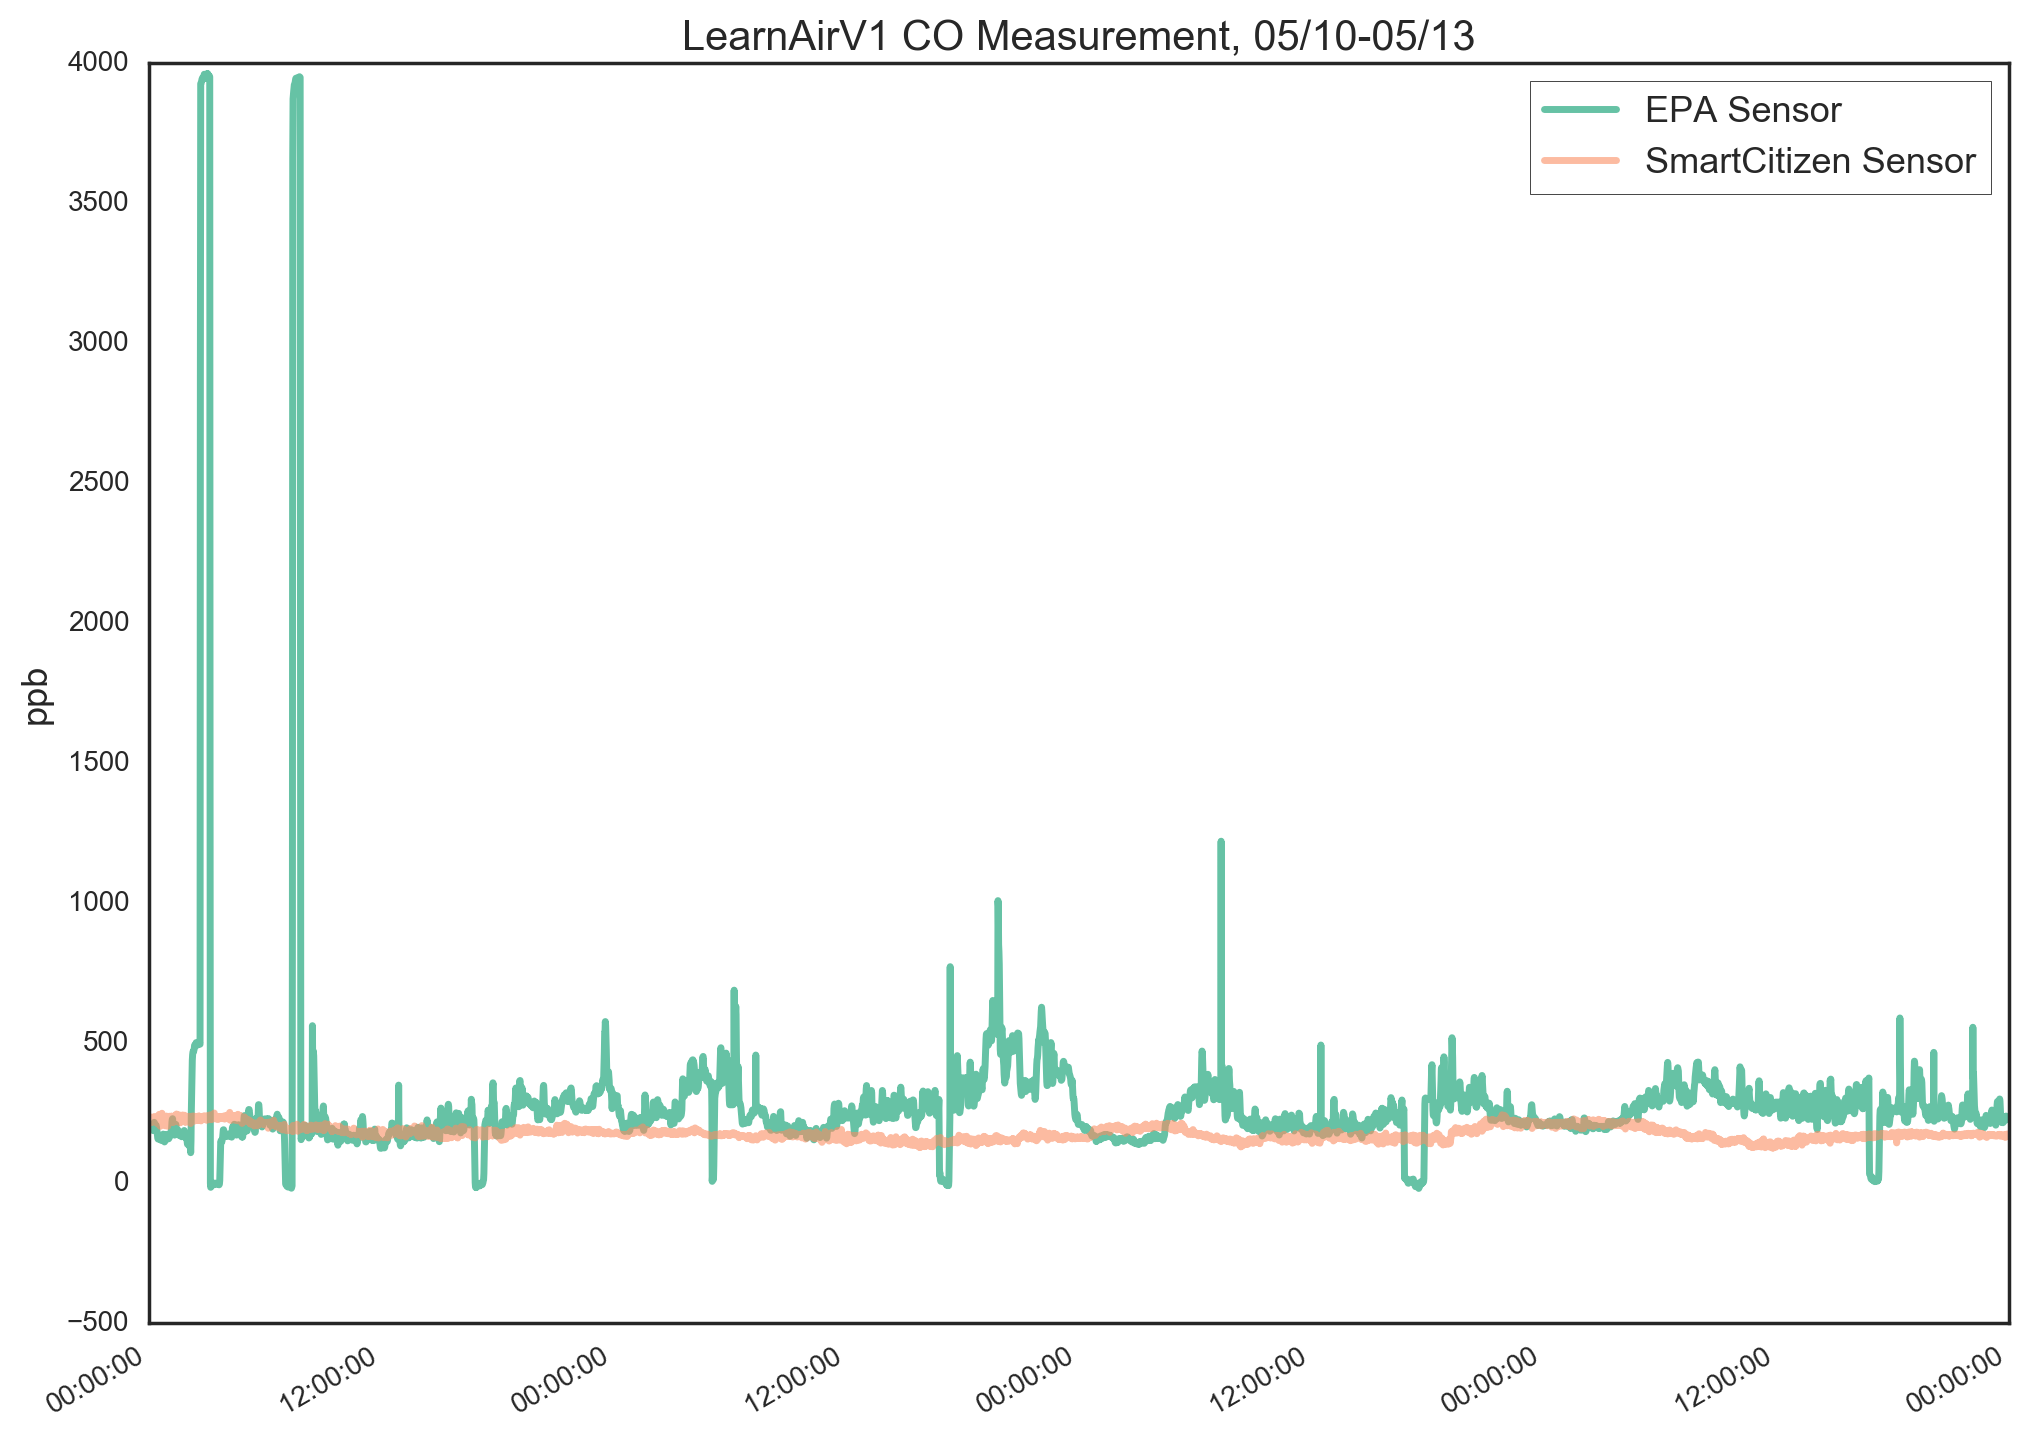
\includegraphics[width=\textwidth]{figs/co_sck_zoomed}               
 	 \caption{SmartCitizen CO Raw Data (orange) vs. EPA reference (green)}
  	\label{fig:sck_co_raw_zoomed}
\end{marginfigure}

The SmartCitizen CO sensor data comes uncalibrated, as a mV value that should correlate to CO concentration.  The first step was to run a bounded LMSE minimization on the data in order to scale and offset it appropriately to match the real data.  You can see the final result of such a scaling in Figure \ref{fig:sck_co_with_7p5_accuracy_zoomed}.  You'll notice that the LMSE minimization basically scaled the sensor values down to a minimal amount of variation.  This suggests that the sensor data itself is relatively useless in this context, which is relatively unsurprising given its working range and the near constant <1 ppm exposure.  

Interestingly, the SCAQMD (South Coast Air Quality Management District) showed good correlation for 5-minute average, 500-1000 ppb range over their ten day co-location study.  Our measurements were a few hundred ppb lower on average.  It's also unclear which version of the Smart Citizen sensor SCAQMD tested, as Smart Citizen released an updated version of their board with completely different CO and NO2 gas sensors.  It appears likely, given the test date, that they were using a different (though similarly priced) sensor module entirely.


\FloatBarrier
\subsection{Machine Learning}


Machine learning on this data will tell us effectively nothing about the sensor's accuracy, since the sensor's correlation to the correct values is so poor.  We don't need machine learning to see that the sensor has failed to predict meaningful values.  Instead, applying machine learning here reduces to a comparison of the real CO concentration to a (more or less) constant baseline-- this means our machine learning techniques simply attempt to predict when transients and elevated levels of CO occur at this location using metrological and other sensor data. 


\begin{figure}[htb]
 	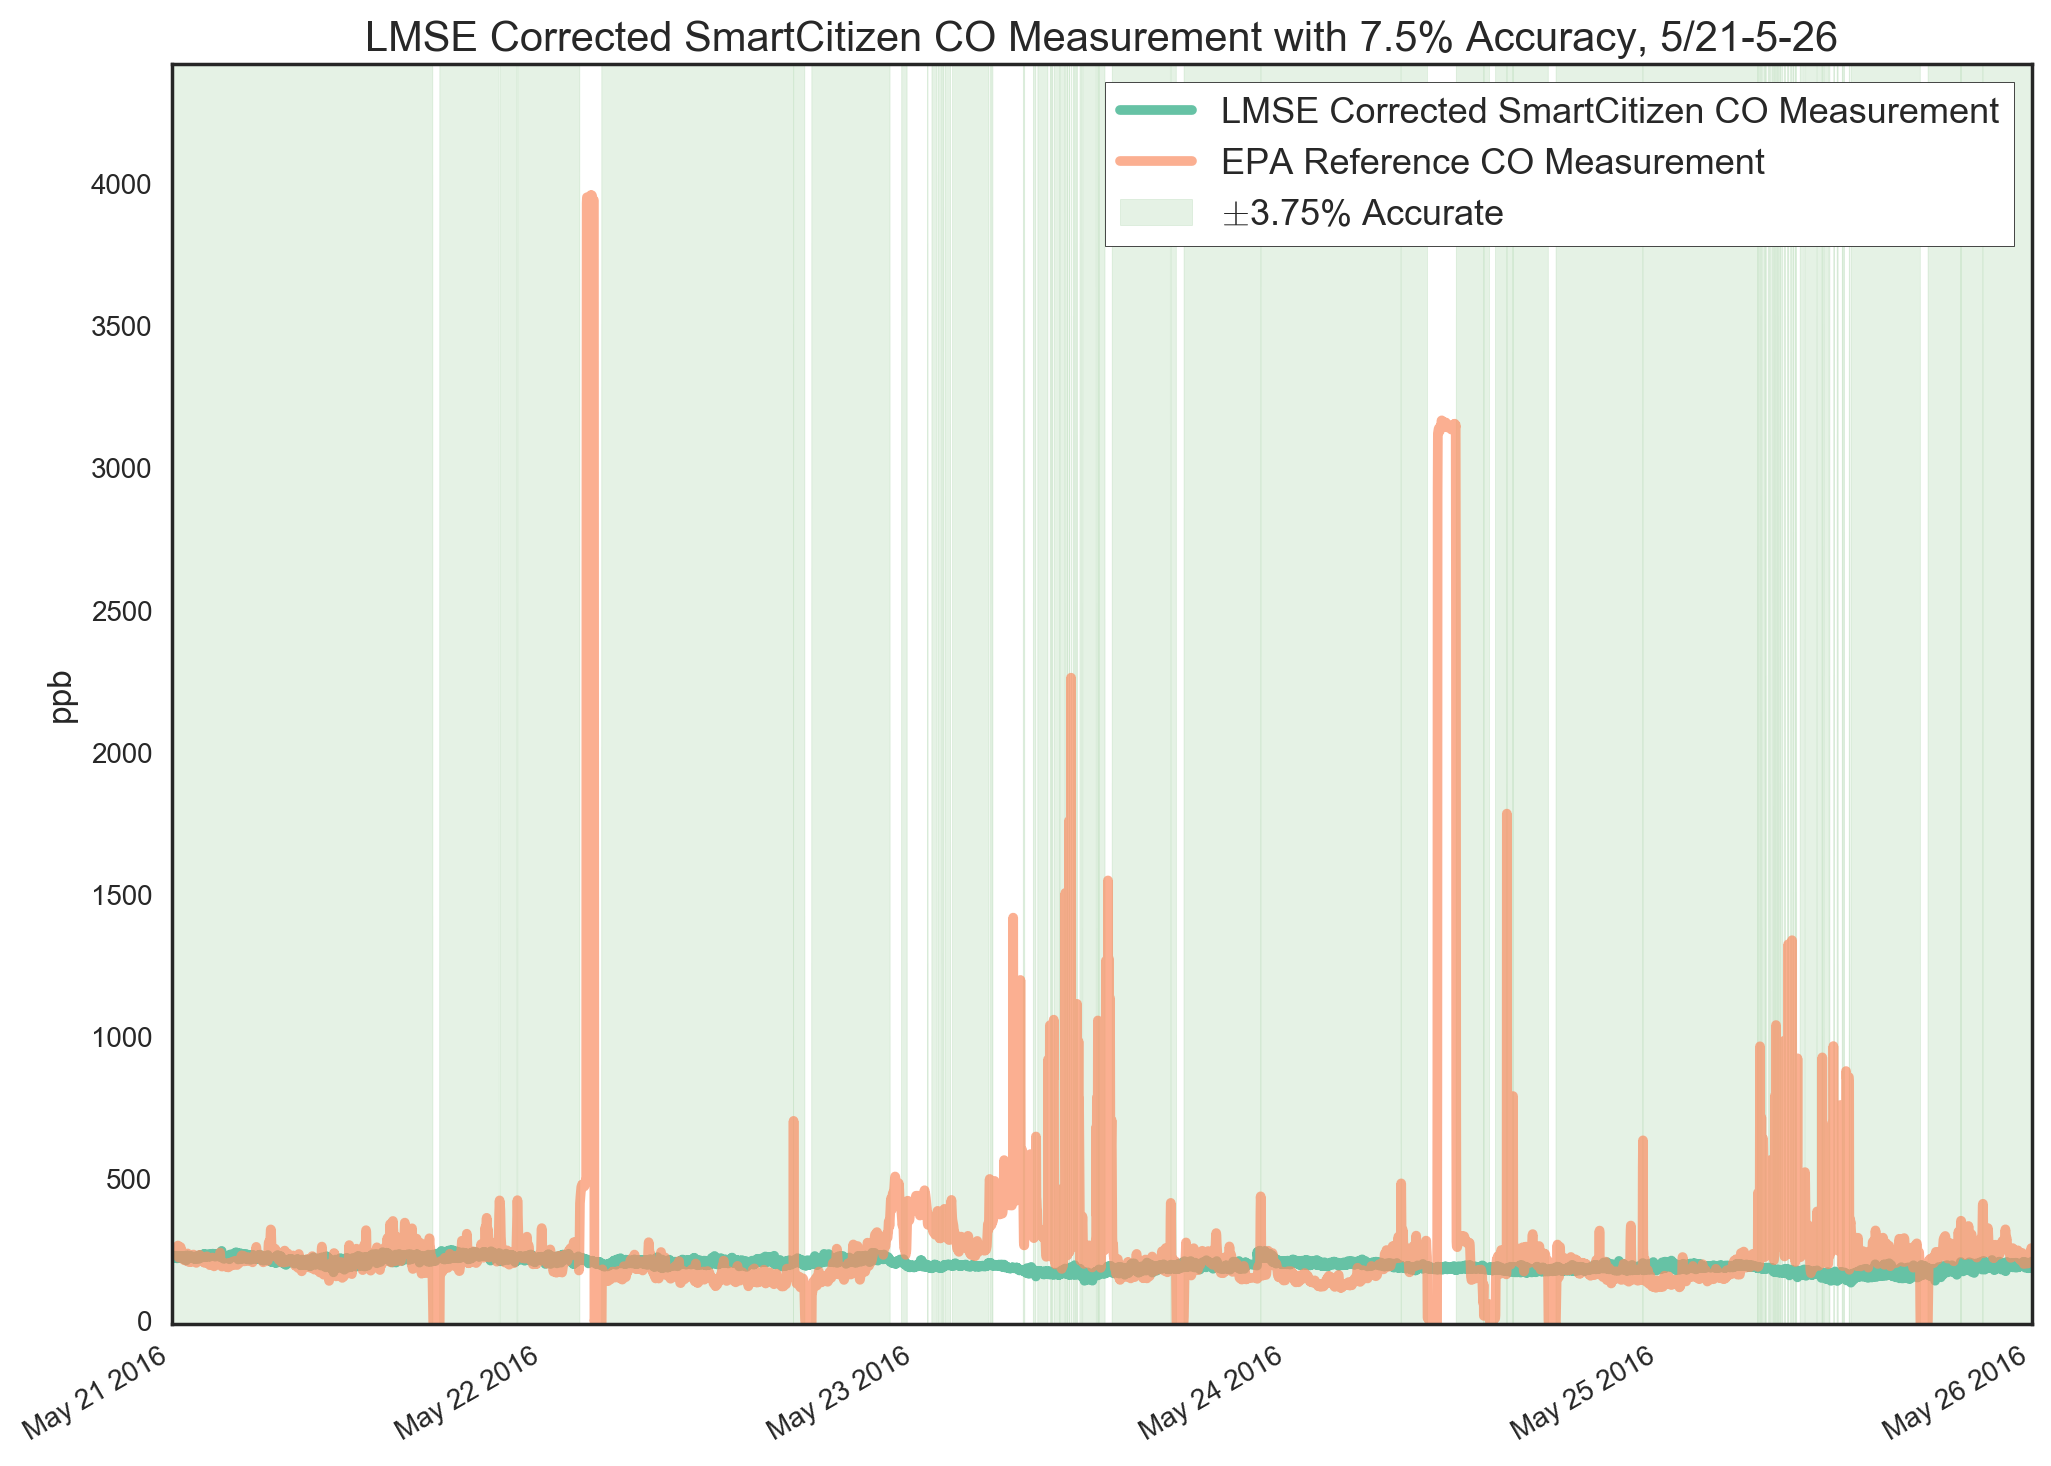
\includegraphics[width=\textwidth]{figs/sck_co_with_7p5_accuracy_zoomed}               
 	 \caption{SmartCitizen CO with 7.5\% Accuracy Threshold}
  	\label{fig:sck_co_with_7p5_accuracy_zoomed}
\end{figure}

In this case, the threshold for an `accurate' reading made by the SmartCitizen CO sensor was set at 7.5\% (or $\pm$3.75\%) of the full range of values detected for the actual CO levels, ~315 ppb ($\pm$157.5 ppb).   Figure \ref{fig:sck_co_with_7p5_accuracy_zoomed} shows the Smart Citizen values against the reference, with `accurate' measurements highlighted with a green background.  The `inaccurate' readings are the peaks and large diversions from the baseline.

As with all of the machine learning models, scikit learn was used to conduct a parameterized search for the optimal logistic regression was conducted using parameters C = [0.001, 0.1, 10, 1000] and penalty-type=['L1', 'L2'] with a 2-fold cross-validation.  This covers a reasonable amount of parameter space for the minimal 16 rounds of training and validation (~1-2 hours on my i5 laptop).  For this test, an L1 penalty and C=10 regularization term gave the best ROC\_AUC score of 0.82.  


\begin{table}[]
\centering
\begin{tabular}{|c|c|c|c|c|}
\toprule
\multicolumn{5}{|c|}{Error Rates for SmartCitizen CO with Logistic Regression} \\
&\multicolumn{2}{|c|}{all features} & \multicolumn{2}{|c|}{top 15 features} \\
&shuffled & chunked & shuffled & chunked \\
avg & 0.09 & 0.09 & 0.09 & 0.09 \\
min & 0.08 & 0.03 & 0.09 & 0.08 \\
max & 0.09 & 0.12 & 0.09 & 0.11 \\
\bottomrule
\end{tabular}
\label{tab:sck_co_error_rates}
\caption{Error Rates for Predicting SmartCitizen CO Accuracy with Logistic Regression}
\end{table}

We see similar error rates of about 9\% error in our predictions regardless of whether we chunk or shuffle the data, or whether we use the full set of ~150 features or just a subset of the top fifteen.  The average confusion matrix (five shuffled trained sets validated on a new 1/5 of the full data-set each time) is shown in Table \ref{tab:sck_co_confusion}.  The confusion matrix for the chunked set has similar values.

\begin{margintable}[]
\centering
\offinterlineskip
\hspace*{-5cm}\raisebox{-4cm}[0pt][0pt]{\rotatebox[origin=c]{90}{\parbox[c][0pt][c]{3cm}{\textbf{Actual Values}\\[20pt]}}}\par
\hspace{.3cm}\MyHBox[\marginparwidth]{Predicted Values}\par
\vspace{-.5cm}
\hspace*{1cm}\MyHBox{0}\MyHBox{1}\par
\MyTBox{0}{197.0}{1187.4}
\vspace{-.35cm}\MyTBox{1}{108.6}{13499.2}\raisebox{-1cm}
}
\label{tab:sck_co_confusion}
\caption{Average SmartCitizen CO Confusion Matrix w/Shuffled K-Fold}
\end{margintable}

Though these conditions look the same based on average error rate and confusion matrix, when we examine the confidence of our predictions we see some dramatic differences in the shuffled vs. chunked cases.  From Figure \ref{fig:sck_co_7p5_roc} we can see the shuffled tests resulted in strong, consistent AUC-ROC scores between 0.81 and 0.83, while the chunked version resulted in unconvincing, highly variable results from 0.43 (worse than uneducated guessing) to 0.76.  When using only the top 15 features from a random tree algorithm, we see similar trends, however our accuracy drops from slightly above 0.8 to slightly about 0.7 for the shuffled case (see Appendix D for a list of the top features selected in this way, and a graph of ROC results for the same algorithm using just those features).   

\begin{figure}[htb]
 	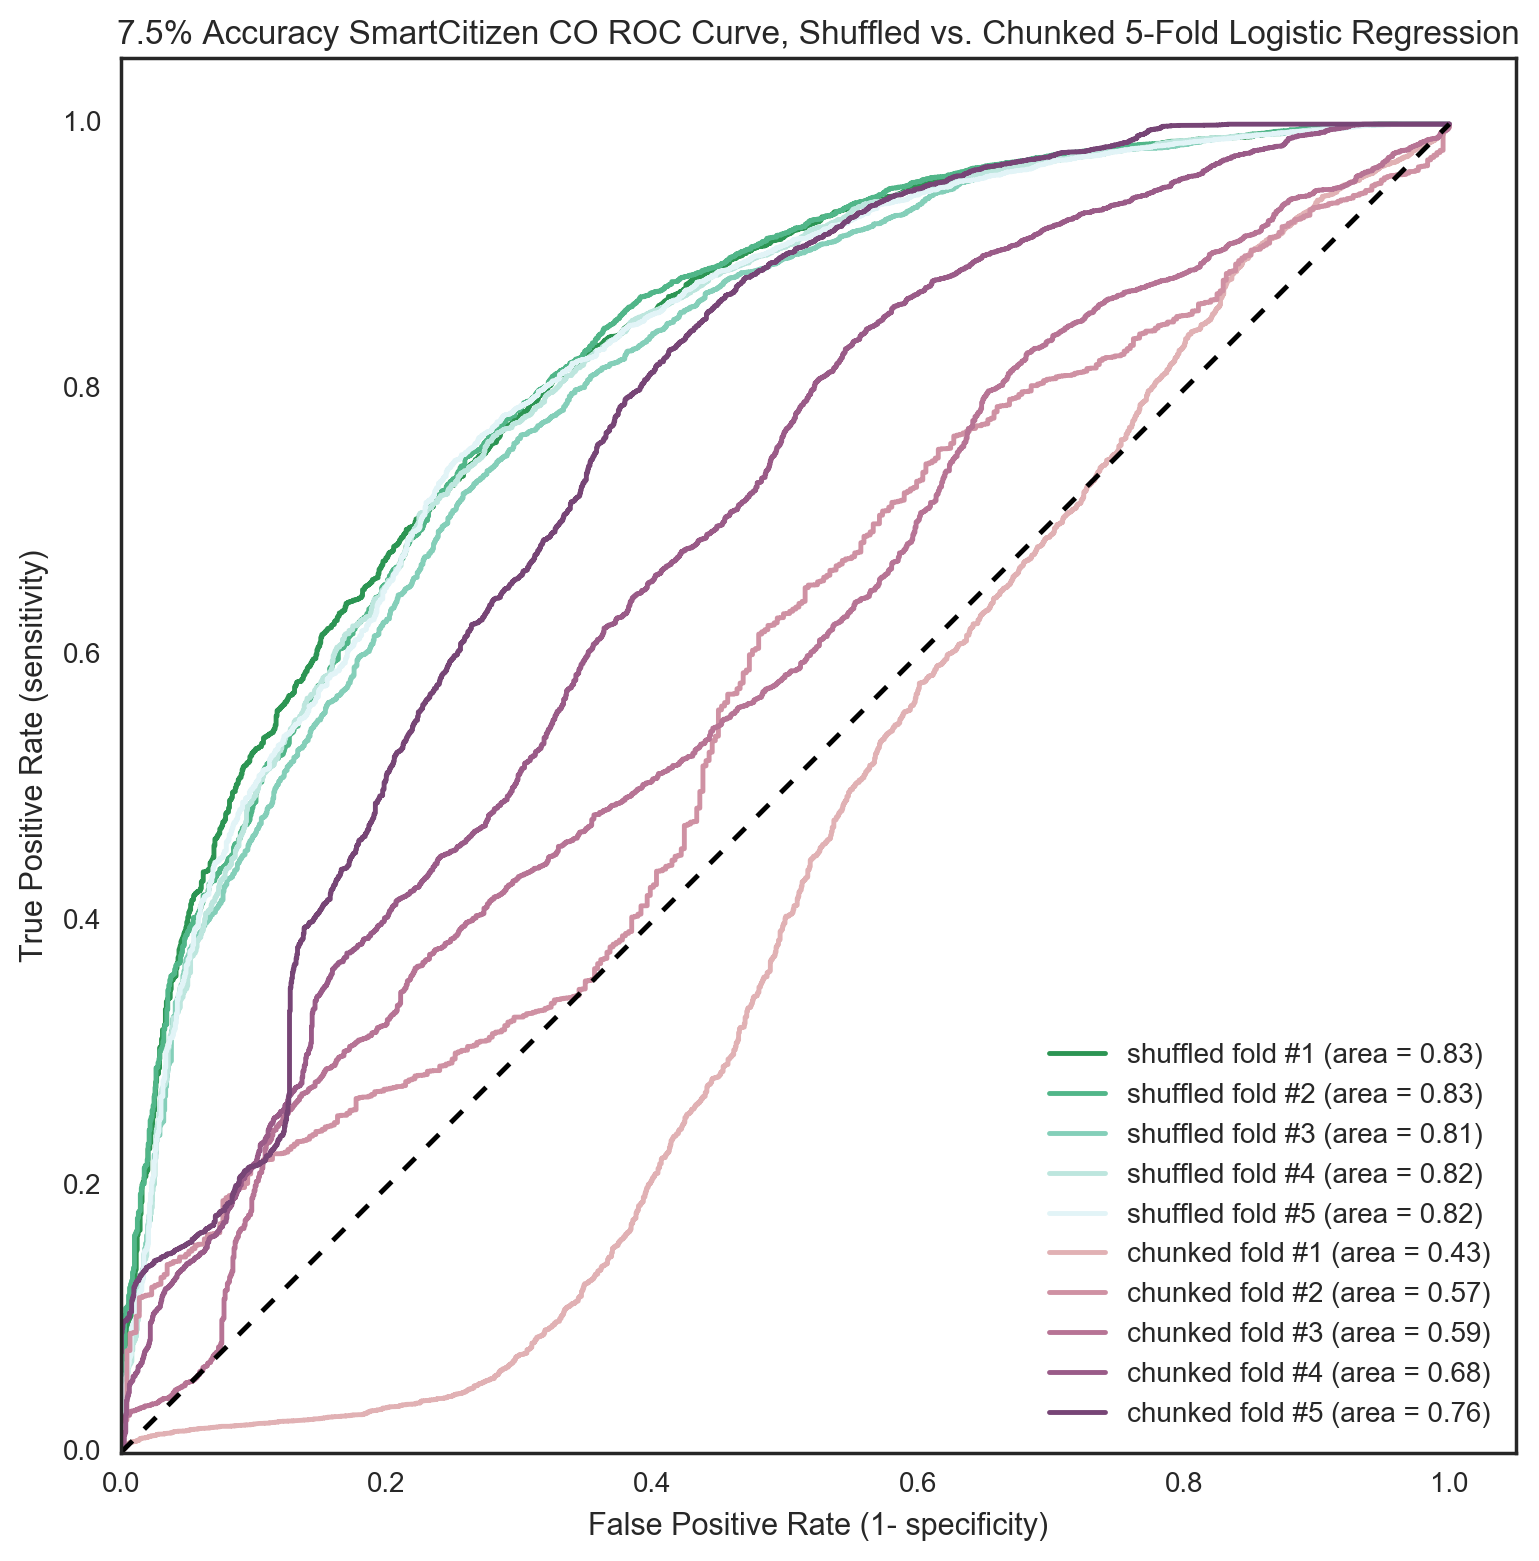
\includegraphics[width=\textwidth]{figs/sck_co_7p5_roc}               
 	 \caption{SmartCitizen CO ROC Curve}
  	\label{fig:sck_co_7p5_roc}
\end{figure}

\begin{table}[]
\centering
\small
\begin{tabular}{lllllllll}
\\
\\
\toprule
     & Corr. & Lasso & Lin Reg & RF   & RFE  & Ridge & Stability & Mean \\
\midrule
bkcarbon                            & 1     & 0          & 0    & 1    & 0.58  & 0.28      & 0.93 & 0.54 \\
avg\_60\_bkcarbon                   & 0.98  & 0          & 0    & 0.25 & 0.53  & 0.15      & 0.83 & 0.39 \\
evening                             & 0.17  & 0          & 0.07 & 0.19 & 0.82  & 0.18      & 1    & 0.35 \\
avg\_1440\_bkcarbon                 & 0.57  & 0          & 0    & 0.37 & 0.53  & 0.44      & 0.54 & 0.35 \\
humidity\_box\_differential         & 0.1   & 0          & 0.01 & 0.22 & 1     & 1         & 0.02 & 0.34 \\
afternoon                           & 0.17  & 0          & 0.07 & 0    & 0.84  & 0.19      & 1    & 0.32 \\
avg\_60\_forecastio\_humidity       & 0.01  & 0          & 0.01 & 0.12 & 1     & 1         & 0    & 0.31 \\
temp\_sck\_box\_differential        & 0.09  & 0          & 0    & 0.45 & 0.84  & 0         & 0.73 & 0.3  \\
Solar Panel ( V)                    & 0.05  & 0          & 1    & 0    & 0.77  & 0         & 0    & 0.26 \\
avg\_720\_bkcarbon                  & 0.65  & 0          & 0    & 0.26 & 0.27  & 0.14      & 0.43 & 0.25 \\
forecastio\_apparentTemperature     & 0.04  & 1          & 0    & 0.03 & 0.16  & 0         & 0.43 & 0.24 \\
lmse\_avg\_30\_scaled\_arduino\_ws  & 0     & 0          & 0    & 0.05 & 0.8   & 0.03      & 0.79 & 0.24 \\
forecastio\_clear-night             & 0     & 0          & 0.08 & 0.04 & 0.91  & 0.06      & 0.51 & 0.23 \\
forecastio\_partly-cloudy-day       & 0.06  & 0          & 0.08 & 0    & 0.91  & 0         & 0.55 & 0.23 \\
forecastio\_partly-cloudy-night     & 0.01  & 0          & 0.08 & 0    & 0.89  & 0.06      & 0.54 & 0.23 \\
avg\_30\_scaled\_arduino\_ws        & 0     & 0          & 0.02 & 0.07 & 0.81  & 0         & 0.74 & 0.23 \\
Noise ( mV)                         & 0.02  & 0          & 0    & 0.11 & 0.39  & 0.02      & 0.92 & 0.21 \\
avg\_720\_lmse\_scaled\_sharpDust   & 0.03  & 0          & 0    & 0.15 & 0.55  & 0.22      & 0.52 & 0.21 \\
derivative\_avg\_720\_bkcarbon      & 0     & 0          & 0    & 0.12 & 0.63  & 0.25      & 0.45 & 0.21 \\
daily\_avg\_sck\_humidity           & 0.07  & 0          & 0    & 0.18 & 0.59  & 0.17      & 0.4  & 0.2  \\
derivative\_avg\_360\_lmse\_as\_no2 & 0     & 0          & 0    & 0.11 & 0.55  & 0.73      & 0    & 0.2  \\
derivative\_avg\_1440\_bkcarbon     & 0.02  & 0          & 0    & 0.14 & 0.64  & 0.02      & 0.58 & 0.2  \\
evening\_rush                       & 0.13  & 0          & 0    & 0.04 & 0.49  & 0.1       & 0.54 & 0.19 \\
avg\_60\_forecastio\_pressure       & 0.07  & 0          & 0    & 0.26 & 0.41  & 0.01      & 0.6  & 0.19 \\
\bottomrule
\end{tabular}
\label{tab:sck_co_top_features}
\caption{Top Features for Predicting SmartCitizen CO}
\end{table}

Table \ref{tab:sck_co_top_features} shows the top features for predicting CO variations away from the baseline, as determined by seven different feature reduction techniques.   

The top features-- combined with our ROC results-- give us insight into the usefulness of this algorithm for predicting transient fluctuations in CO.  The large divergence between shuffled and chunked data suggests we have not collected enough data yet to make seasonally-agnostic predictions in CO.  However, the promising results in our shuffled data lead us to believe it is possible to make fairly robust predictions (within or accounting for the season) with enough data collection.  The relationships we find in our shuffled results are consistent and reliable across test sets.  

The top features include black carbon readings, time of day designations (like evening or night), windspeed measured at the sensor, and temperature.  These are in line with expectation-- as a similar combustion byproduct, we would expect black carbon and CO to be closely related.  Heavy traffic (the main source of both black carbon and CO) has predictable time-of-day patterns.  Temperature and windspeed have been directly correlated to changes in CO concentration, given a constant, predictable source.   Furthermore, we'd expect our prediction to be based on a complex relationship of many underlying features.  The difference in results from the full feature set to the reduce set corroborates this assumption.   

In our test, the SmartCitizen CO sensor provided no meaningful data when compared and fit against the FRM reference.  This changed our machine learning task from a `predict sensor accuracy' problem to a `predict CO transient' one.  Our results indicate a strong likelihood of making good predictions of transient events for CO with a high quality black carbon sensor as part of the device.  However, these predictions are complex, and require a lot of diverse sensor data to tease out a strong prediction.  Furthermore, this relationship appears to be seasonally dependent, and thus an extensive training set-- longer than the two month season change we captured here-- is necessary to predict CO transient behavior with good accuracy.

See Appendix D for more plots outlining the LMSE pre-processing steps, other accuracy thresholds we attempted, a plot of the SmartCitizen data with a correct/incorrect prediction overlay, and the Random Tree reduced-feature selection table and corresponding ROC curves. 

%http://www.aqmd.gov/docs/default-source/aq-spec/field-evaluations/smart-citizen-kit---field-evaluation.pdf?sfvrsn=2